
\section{Experimental results}
\label{sec:exp}

%\fcomment{Need to present here both practical results that illustrates the outcome of our solution and how it benefits ... eg show a case where new goals are introduced as we go along.
%Also need some analysis -- potentially numerical -- on the overhead and impact fo both solutions relative to each other but also potentially to a more direct classic approach. 
%To finally discuss why one solution was preferred on our system} 

Our experiment follows that of the original plan given in
Fig. \ref{fig:ex:plan}. At the beginning, the AUV need to {\em Sample Vent2}
and it has to return to the surface by the end of the mission. We
implemented this on our executive with plans being produced by the
europa planning engine \cite{frank2003}.\fcomment{I think it is
  important to give at least dome indication of the kind of tools used.
  this should be enough as it is not really giving away that we used
  trex}. Figure \ref{fig:ex:mixed1}
demonstrates the resulting plan from our algorithm and will guide our
explanation. Both algorithms will result in the same execution of the
plan but their approach is quite different.

\begin{figure}
  \centering
  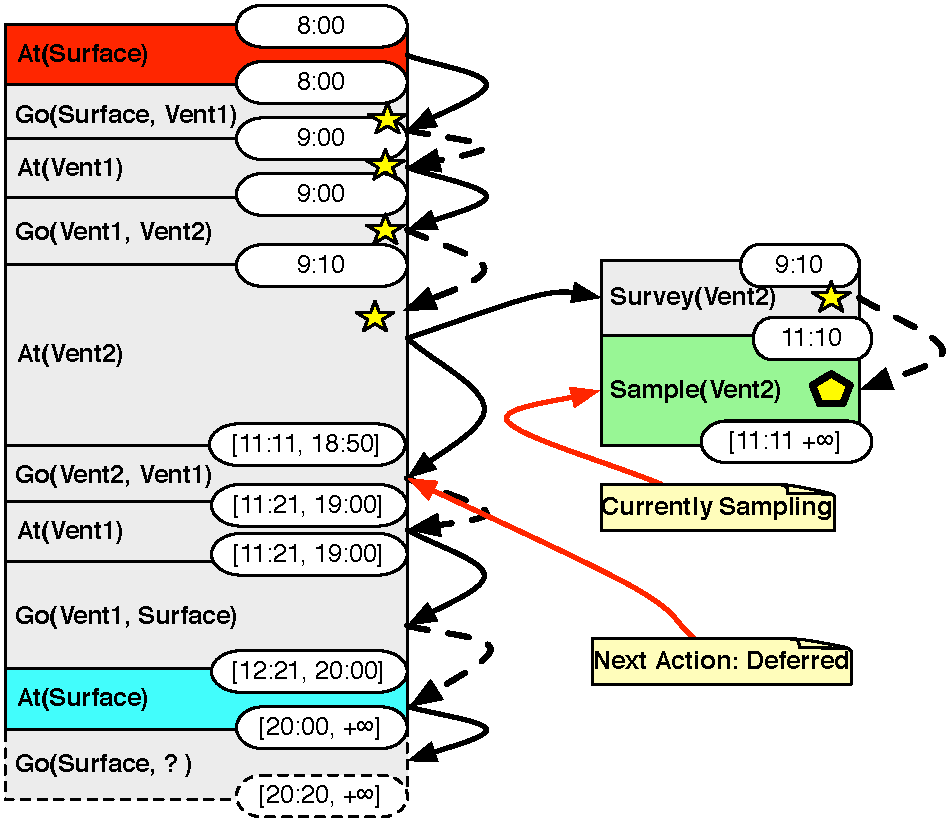
\includegraphics[width=0.8\columnwidth]{figs/example_MixedInitial}
  \caption{\small The algorithmic solution for the plan from
    Fig. \ref{fig:ex:plan}. Solid lines indicate conditions and
    dashed lines indicate effects. Pentagons indicate {\em urgent}
    goals, stars indicate tokens that were deduced as {\em proactive}.}
  \label{fig:ex:mixed1}
\end{figure}

For Algorithm \ref{DispatchToken}, the search is quite straight
forward. For example in Fig. \ref{fig:ex:mixed1}, if we are {\em At
Surface} then the next {\em Go} token will be dispatched. Because the
search will follow the causal links forward, where upon, it will find
the goal {\em Sample Vent2} resulting in dispatching proactively.
Similarly, this happens for all of the tokens that are starred. The
next token to {\em Go} to {\em Vent1} is continuously searched but deferred for later dispatching,
because it is not connected to a goal. The resulting
AUV stays at {\em Vent2} rather than heading to the {\em Surface}
immediately like in Fig. \ref{fig:ex:proactive}.

For the distributed algorithm approach, each token is checked during
the creation of the plan to see if it is an external goal in
$\Phi_{ge}$, or connected to one through a causal link. When the {\em
Sample Vent2} is checked, we immediately find that it is a goal. We then
follow the reverse causal link and find {\em Survey Vent2}.  However to
better illustrate the algorithm, we can imagine that only the {\em Survey
Vent2} has been causally connected to the goal so far. Therefore, we
only star those two tokens. The path from {\em Surface} to {\em Vent1}
to {\em Vent2} has yet to be built. When the path has finally been
built, and {\em At Vent2} is checked, our algorithm searches one
causal link and finds {\em Survey Vent2} which is starred. The search
then follows the reverse causal link and stars the rest of the
path. The starred tokens will then be proactively dispatched while the
non-starred tokens will be deferred until later. Having similar
results to Algorithm \ref{DispatchToken}.

\begin{figure}
  \centering
  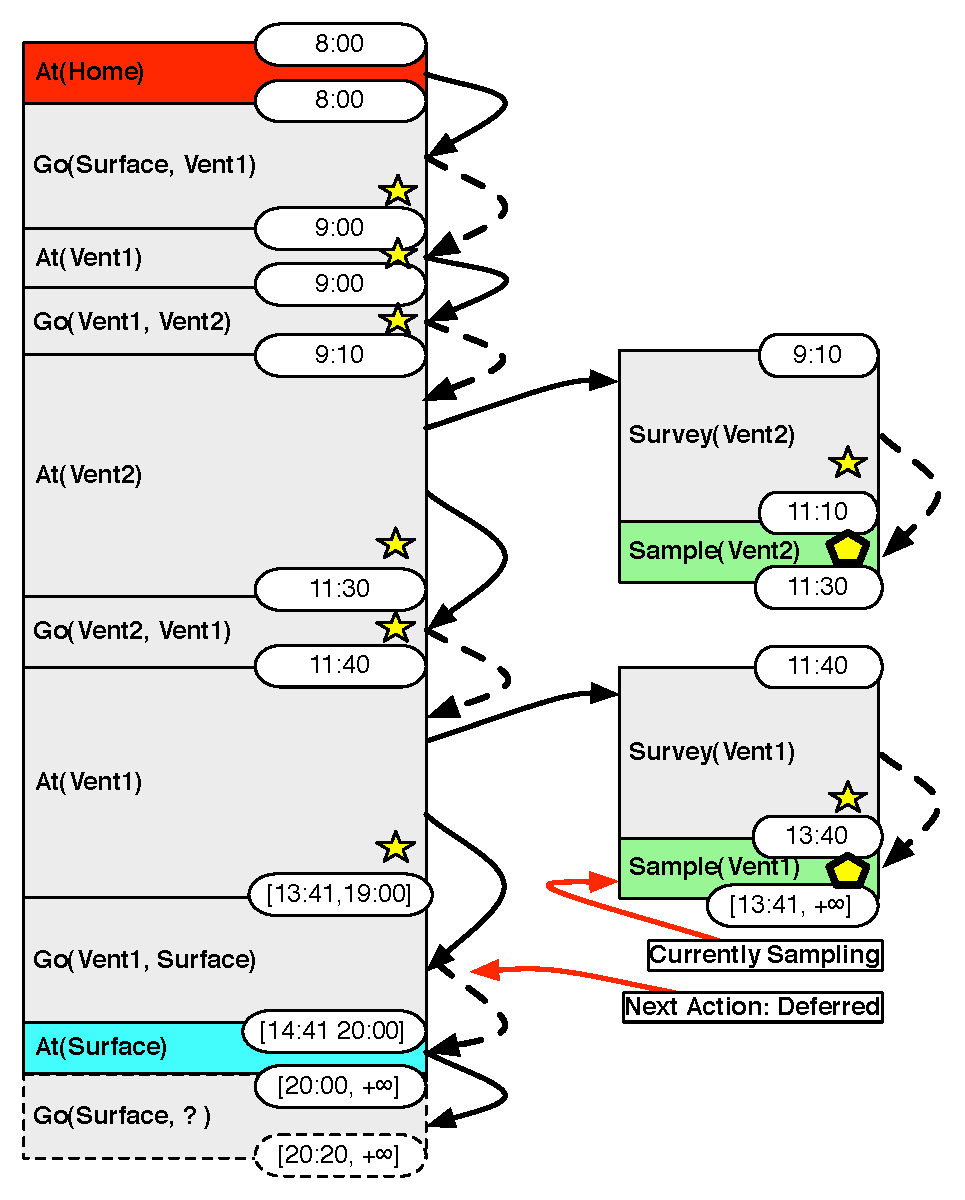
\includegraphics[width=0.8\columnwidth]{figs/example_MixedUpdate}
  \caption{\small The solution after receiving external request for
    the plan from Fig. \ref{fig:ex:mixed1}} 
  \label{fig:ex:mixed2}
\end{figure}

Our reasoning for keeping the AUV at {\em Vent2} is that
nothing is requiring it to go {\em Surface} as soon as possible and that
more external requests may come in the near future. To demonstrate
this imagine that while the AUV is at {\em Vent2} it gets a
request at 11:30 asking it to {\em Sample Vent1}.  We show the resulting plan in
Fig. \ref{fig:ex:mixed2}. Again, both algorithms will result in the
same conclusion. Algorithm \ref{DispatchToken} will search from {\em
Go(Vent2, Vent1)} and will now find {\em Sample Vent1}. The
distributed algorithm will find and star the new tokens when the plan
gets updated. The resulting new starred tokens will be proactively
dispatched.

As the end of the day approaches, the AUV will need to start heading
to the surface. At 19:00 both algorithms will find that the {\em Go(Vent1,
Surface)} is still not connected to a goal but that the upper bound time
for starting the token has been reached. Therefore, we will dispatch
the token because it has become necessary for completing the plan.
After returning to the {\em Surface}, the plan shows that the AUV will then {\em
Go(Surface, ?)} (dashed in the figures). This is an artifact resulting
from the plan model which specifies that a {\em At} token is followed by a {\em Go}. 
However, our algorithm will not be dispatching this token as 
it is not connected to a goal and its upper bound start time
($+\infty$) will not be met.

\begin{figure}
\centering
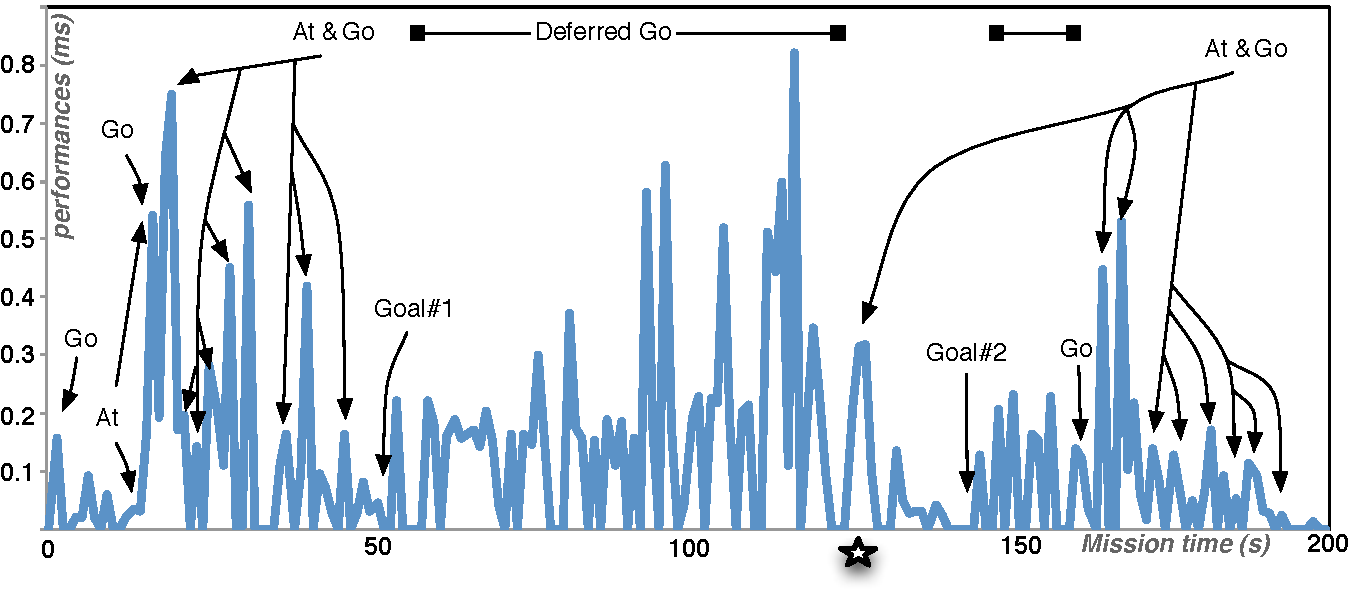
\includegraphics[width=\columnwidth]{figs/example_run.pdf}
\caption{\small  One mission run that shows the time needed for dispatching. Star represents when the Goal\#2 was
received and integrated into the plan. Lines with boxes at the end represent the deferred action {\em Go} Because of space,
we didn't put an arrow to every {\em At}. Our concern were the peak that showed where the system had to dispatch both {\em At} and {\em Go}. } 
  \label{fig:example_run}
\end{figure}

In our experiments, the simulated AUV missions ran in a virtual machine running Ubuntu, a Linux distribution. The virtual machine
was run on a MacBook Pro. The virtual machine was allocated one processor from a 2.33 GHz Intel Core 2 Duo processor. 

In Figure \ref{fig:example_run}, we show a simulated mission run that is similar to our original example in Fig. \ref{fig:ex:plan}.
However, in order to increase the complexity of the plan we added a total of ten locations, eight before the vents. The first goal 
is to sample {\em vent2} at location ten and the second is to sample {\em vent1} at location nine. The spikes in the time 
happen when it dispatches both an {\em At} and a {\em Go} which means that the graph must be searched twice. There
is a clear trend that as the AUV gets closer to the goals the time decreases because the search distance decreases. 
However, there is some variability in the time which can most likely be accounted for as timing with context switching as the virtual
machine only has one processor. Before Goal\#2 is integrated into the plan at time 127, the algorithm is continually
searching the graph which is shown as the time is on an average above .2 milliseconds. At tick 127, the {\em Go} is no longer 
deferred and gets dispatched. The search for Goal\#2 becomes relatively simple as it is not very far away in the plan, and thus the
time decreases significantly.

\begin{figure}
\centering
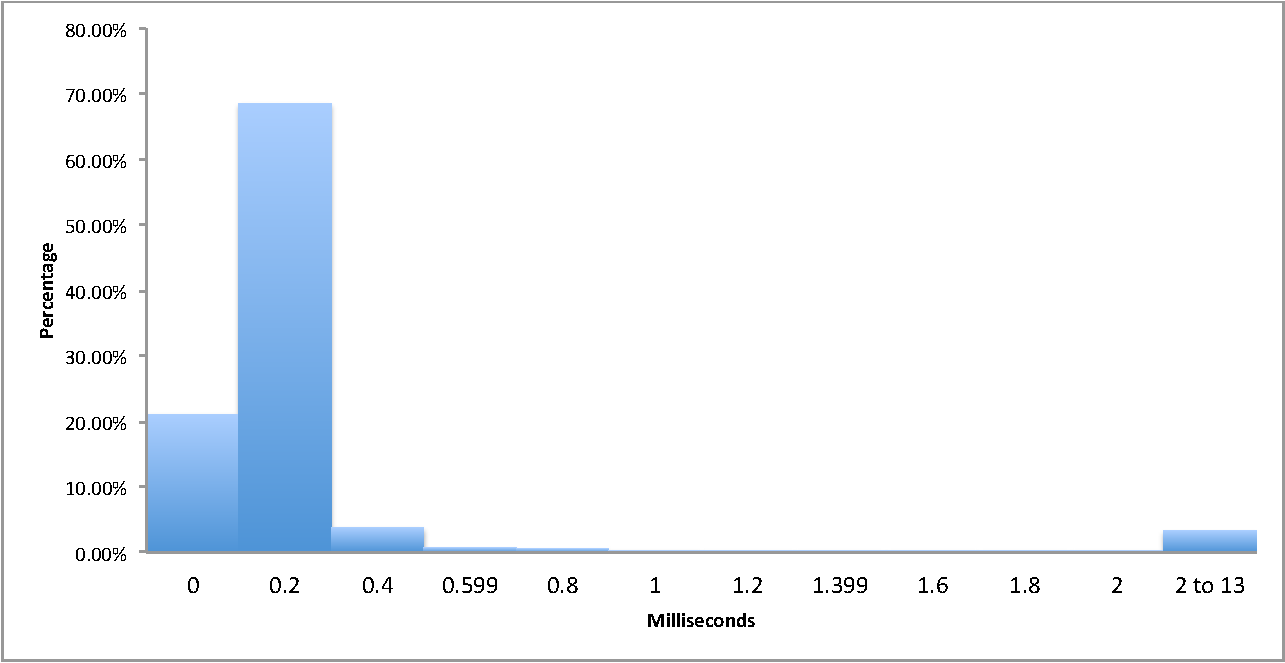
\includegraphics[width=\columnwidth]{figs/HistogramAlg1}
\caption{\small  We ran 500 missions were Algorithm \ref{DispatchToken} was timed for every tick of the mission time.
One goal was inserted into the plan at a random time. Shows the distribution of the time.} 
  \label{fig:histogram}
\end{figure}

In order to demonstrate the average amount of time that Algorithm \ref{DispatchToken} uses, we ran 500 simulated missions
and timed it at every mission tick. Figure \ref{fig:histogram} shows that for about 90\% of the time, Algorithm \ref{DispatchToken}
takes less than .2 milliseconds to complete it's search. The histogram is clearly skewed to the left and decreases quickly as the
time increases. Less than 5\% of the time did Algorithm \ref{DispatchToken} go above
two milliseconds with an upper bound time of thirteen. However, this portion of the histogram is largely condensed in 
order to maintain a reasonable size and would decrease if spread out.   





%%% Local Variables: 
%%% mode: latex
%%% TeX-master: "aaai13"
%%% End: 
